\begin{appendices}
\chapter{近简并能带的朗道量子化条件的证明}\label{app:quantizationruleproof}

在本附录里,我们将要导出近简并能带的朗道能级的量子化条件。我们假设能带在每个$\bk$点都是$D$重近简并的。对于$D=2$,我们已经在\qq{eq:rule}{berryconn}给出了量子化条件;这里,我们要把这样的量子化条件扩展到$D>2$。尽管$D>2$比$D=2$罕见一些,一些具有非点式对称性的材料往往存在着$D>2$的近简并的能带。比如说在具有螺旋轴和时间反演对称性,并且自旋轨道耦合较弱的材料中,高对称面(比如对于螺旋轴$\mathfrak{c}_{2z,\boldsymbol{c}/2}$而言的$k_z=\pi$平面)往往存在着四重近简并。

量子化条件的推导基于一个有效的哈密顿量的WKB近似解。在推导期间,我们需要理解近似所带来的误差,在这里,我们采用大O和小o来量化误差,这两个符号在这里的定义是: 
\begin{itemize}
    \item 
    \begin{equation}
        f(\boldsymbol{x})\sim\text{O}(\{g_i(\boldsymbol{x}), i\in 1..N\})
    \end{equation}
    当 $\boldsymbol{x}\to\boldsymbol{0}$ 定义为 $\exists C>0$ 并且 $\exists \delta>0$ 对于所有的 $\boldsymbol{x}$ 以及 $||\boldsymbol{x}||_\infty<\delta$ 都有
    \begin{equation}
        |f(\boldsymbol{x})|<C\text{max}\{|g_i(\boldsymbol{x})|, i\in 1..N\};
    \end{equation}
    \item 
    \begin{equation}
        f(\boldsymbol{x})\sim\text{o}(\{g_i(\boldsymbol{x}), i\in 1..N\})
    \end{equation}
    当 $\boldsymbol{x}\to\boldsymbol{0}$ 定义为 $\forall \epsilon>0,~\exists \delta>0$ 对于所有的 $\boldsymbol{x}$ 以及 $||\boldsymbol{x}||_\infty<\delta$,
    \begin{equation}
        |f(\boldsymbol{x})|<\epsilon\text{max}\{|g_i(\boldsymbol{x})|, i\in 1..N\}.
    \end{equation}
\end{itemize}
这里, $||\boldsymbol{x}||_\infty=\text{max}\{|x_i|\}$。

正如\s{sec:qtznrules}中所述,我们首先需要先将哈密顿量$\hat{H}$分解为$\hat{H}_0$和一个微扰$\delta\hat{H}=\eta\hat{H}_1$。这里的$\eta$是无量纲的小量。我们假设$\eta\hat{H}$微扰地破坏了$\hat{H_0}$的$D$重能带简并。对于二重近简并,正如正文中所述,$\eta$可以选择为$\delta S/S$。

为了近似求解薛定谔方程,我们采用有效哈密顿量理论\cite{rotheffham,100p}。有效哈密顿量是在一组经过磁场修正过的$\hat{H}_0$的本征布洛赫函数展开的\cite{rotheffham}$\{\tilde{\psi}_{n\boldsymbol{k}}\}_{n=1}^D$。如果将本征函数$\phi$写在这组基下($\phi=\sum_{n=1}^D\sum_{\boldsymbol{k}}f_{n\boldsymbol{k}}\tilde{\psi}_{n\boldsymbol{k}}$),那么薛定谔方程就成为
\begin{equation}
(\mathfrak{H}(\boldsymbol{K})-E)\boldsymbol{f}_{\boldsymbol{k}}=0,\label{eq:schrodinger}
\end{equation}
其中$\mathfrak{H}(\boldsymbol{K})$ (也就是有效哈密顿量)是一个 $D\times D$ 的矩阵微分算符。 

一般而言,有效哈密顿量可以以$a/l^2 (\propto B)$以及$\eta$渐近展开,这两个量都是小量,其比值是一个有限值$l^2\eta/a^2$;这里$a$是晶格格矢的长度,我们将$a$下面设为1。有效哈密顿量关于$l^{-2}$和$\eta$最低阶的项是Peierls-Onsager哈密顿量:$\mathfrak{H}_{0}(\boldsymbol{K}):=\epsilon(\boldsymbol{K})$。这个哈密顿量就是这个$D$重简并的能带的色散关系$\epsilon(\boldsymbol{k})$的Weyl对称的Peierls替换($\bk \rightarrow \bK$),其中$\boldsymbol{K}=\boldsymbol{k}+(e/\hbar)\boldsymbol{A}(i\nabla_{\boldsymbol{k}})$。

有效哈密顿量的次低阶项$\mathfrak{H}_{1}(\boldsymbol{K})$由两部分组成:第一部分是广义的塞曼作用的Peierls替换(在不考虑$\delta \hat{H}$的时候),这一部分包括自旋和轨道磁矩对磁场的响应,也包括一项几何的贝里联络的贡献。第二部分是$\delta \epsilon(\bk)$的Peierls替换,$\delta \epsilon(\bk)$是$\hat{H}_1$在$\hat{H}_0$的$D$重简并的空间里的投影。合在一起我们得到
\begin{equation}
\effH_1(\bk) = \eta\delta \epsilon(\bk)+B(M_{z}-g_s\mu_{B}s_{z}/\hbar+e\epsilon_{\alpha\beta}\mathfrak{X}_{\beta}v_{\alpha}). \label{effham1}
\end{equation}
\q{effham1}中的$M_z$, $s_z$, $\mathfrak{X}$ 和 $v$应该在$\hat{H}_0$的$D$重简并的子空间进行计算。上面的式子假设了磁场$B$沿着$-z$方向。

我们在\q{eq:schrodinger}中采用朗道规范,此时$k_x$是一个好量子数。我们现在要在WKB准经典近似的框架下求解薛定谔哈密顿量。最低阶的解(也就是只含$\mathfrak{H}_0(\bK)$的时候),\q{eq:schrodinger}的解是Zil'berman函数\cite{zilberman},用$k_x^0$来标记,
\begin{equation}
    g_{\bk}^\nu=\frac{1}{\sqrt{|v_x^\nu|}}e^{il^2k_x^0k_y}e^{-il^{2}\int k_x^\nu dk_y}\delta_{k_x^0 k_x},\la{zilberman}
\end{equation}
这里$k_x^\nu$是$k_y$的函数,函数关系由$\epsilon(k_x^\nu,k_y)=E$隐式表示出来。$\epsilon(k_x^\nu,k_y)=E$有多个解,我们用$\nu$标记,用上标$\nu$标出的物理量(比如说\q{zilberman}中的$v_x^\nu(\bk)$)应该在$\bk = (k_x^\nu, k_y)$处计算。

我们采用和文献\onlinecite{100p}类似的处理方式,我们要用下面的多分量的波函数假设来求和薛定谔方程
\begin{equation}
\boldsymbol{f}^\nu=\A^\nu\boldsymbol{g}^\nu,\label{wkb-wf}
\end{equation}
其中
\begin{equation}
g_a^\nu=c_{a}^\nu\frac{1}{\sqrt{|v_x^\nu|}}e^{ik^{0}_{x}k_{y}l^{2}}e^{-il^{2}\int k_{x}^\nu dk_{y}}\delta_{k^{0}_{x}k_{x}},~a\in{1..D}
\end{equation}
其中$c_a^\nu$和$\bk$无关,$\A^\nu$是一个以$k_y$为变量的方阵,我们假设其元素$\A_{ab}^\nu$的大小为$\order(1, \eta l^2):=\order(\{1,\eta l^2\})$。根据文献\onlinecite{100p}的方法,我们得到
\e{
[\effH_{0}(\boldsymbol{K})]_{ab}\A_{bc}^\nu g_{c}^\nu=&\A_{ac}^\nu\epsilon_0(\bK)g_{c}^\nu+i\hbar l^{-2} v_{x}^\nu(\partial_{y}\A_{ac}^\nu)g_{c}^\nu\nonumber\\
&+\text{o}(l^{-2}, \eta),
}
以及
\begin{equation}
[\effH_{1}(\bK)]_{ab}\A_{bc}^\nu g_{c}^\nu=[\effH_{1}]_{ab}\A_{bc}^\nu g_{c}^\nu+\text{o}(l^{-2}, \eta).\label{effH1onA}
\end{equation}
在\q{effH1onA}中忽略掉的一项是$i l^{-2}(\partial_{y}A_{ac}^\nu)g_{c}^\nu d\effH_1/dk_x$。假设$\delta\hat{H}$导致的速度变化没有反常的大,那么忽略这一项就是合理的。

此时,薛定谔方程成为了 
\begin{equation}
i\hbar l^{-2} v_{x}^\nu (\partial_{y}\A_{ac}^\nu)  g_{c}^\nu+[\effH_{1}]_{ab}\A_{bc}^\nu g_{c}^\nu=\text{o}(l^{-2}, \eta).
\end{equation}
如果要上式对任意$\mathbf{c}$都成立,那么
\begin{equation}
\hbar\partial_{y}\A_{ac}^\nu=il^{2}[v_{x}^\nu]^{-1}[\effH_{1}]_{ab}\A_{bc}^\nu+{\text{o}(1, \eta l^2)}.
\end{equation}
这个微分方程的解是一个路径有序的矩阵指数:
\begin{equation}
\A^\nu=\overline{\exp}[il^{2}\int\frac{\effH_{1}}{\hbar v_{x}^\nu}dk_{y}]+{\text{o}(1, \eta l^2)},
\end{equation}

我们在准经典的转折点采用硬边界,并且要求波函数\q{wkb-wf}是单值的\cite{100p},那么我们就可以得到\qq{eq:rule}{berryconn};在\q{eq:rule}中,$a$取$1$至$D$。由于几何的贝里相位相关项,\q{eq:prop}在$\hat{H}_0$的简并子空间的基矢变化下是协变的【参见文献\onlinecite{100p}的式133】,因此,$\{\lambda_a\}_{a=1}^D$模$2\pi$是由良好定义的。

由于$\lambda_a$是$\A$在整个磁振子轨道的本征值的相位,$\lambda_a$同样带有一个$\text{o}(1, \eta l^2)$的不确定性。比如说,在面外磁场的Rashba模型中,我们比较了量子化条件和精确解的差别,发现量子化条件缺少了量级为$\eta^2 l^2$的项;换句话说,缺少的项是\q{eq:Rashba-exact}中的正比如 $l^2\delta S^2/S$的项。这些项在我们假设$\eta$和$l^{-2}$很小,并且$l^2\eta$是有限值的情况下是可以忽略的。值得注意的是,$l^2\delta S^2/S\ll 1$和标准的准经典条件,给出了适用我们提出的量子化条件的$B$的上限和下限:$S^{-1} \ll l^2 \ll S/(\delta S)^2$。


除了我们现在所述的有效哈密顿量的处理方法,我们了解到多个相互关联的能带\cite{culcer_coherent_2005}已经有了准经典的波包理论。我们的量子化条件有可能也能从波包理论的再量子化导出\cite{xiao_berry_2010},但是这一点留由以后的工作研究。

\chapter{量子化条件和精确对角化结果的比较}\label{app:approximatevsexact}

这里,我们将要比较精确对角化的朗道能级和量子化条件【\qq{eq:rule}{berryconn}】得到的朗道能级的差异。我们采用的模型是面外磁场下的Rashba-Dresselhaus二维电子气【\fig{fig:error}(a)】,以及倾斜磁场下的Rashba模型【\fig{fig:error}(b)】。这两个模型据我们所知都没有解析解。我们采用$\text{error}:=|\epsilon_\text{rule}-\epsilon_\text{exact}|/\var_c$来量化我们的量子化条件的误差。在我们测试的参数区间内,准经典条件($l^2 S\gg 1$)以及近简并条件($\delta S/S\ll 1$)都成立。正如Rashba二维电子气【参见\q{eq:Rashba-exact}】,我们的量子化条件在$l^2\delta S^2/S$变小的时候精确度更高,可见这一项给出了误差中的主导贡献【参见附录\ref{app:quantizationruleproof}中的讨论】。


\begin{figure}
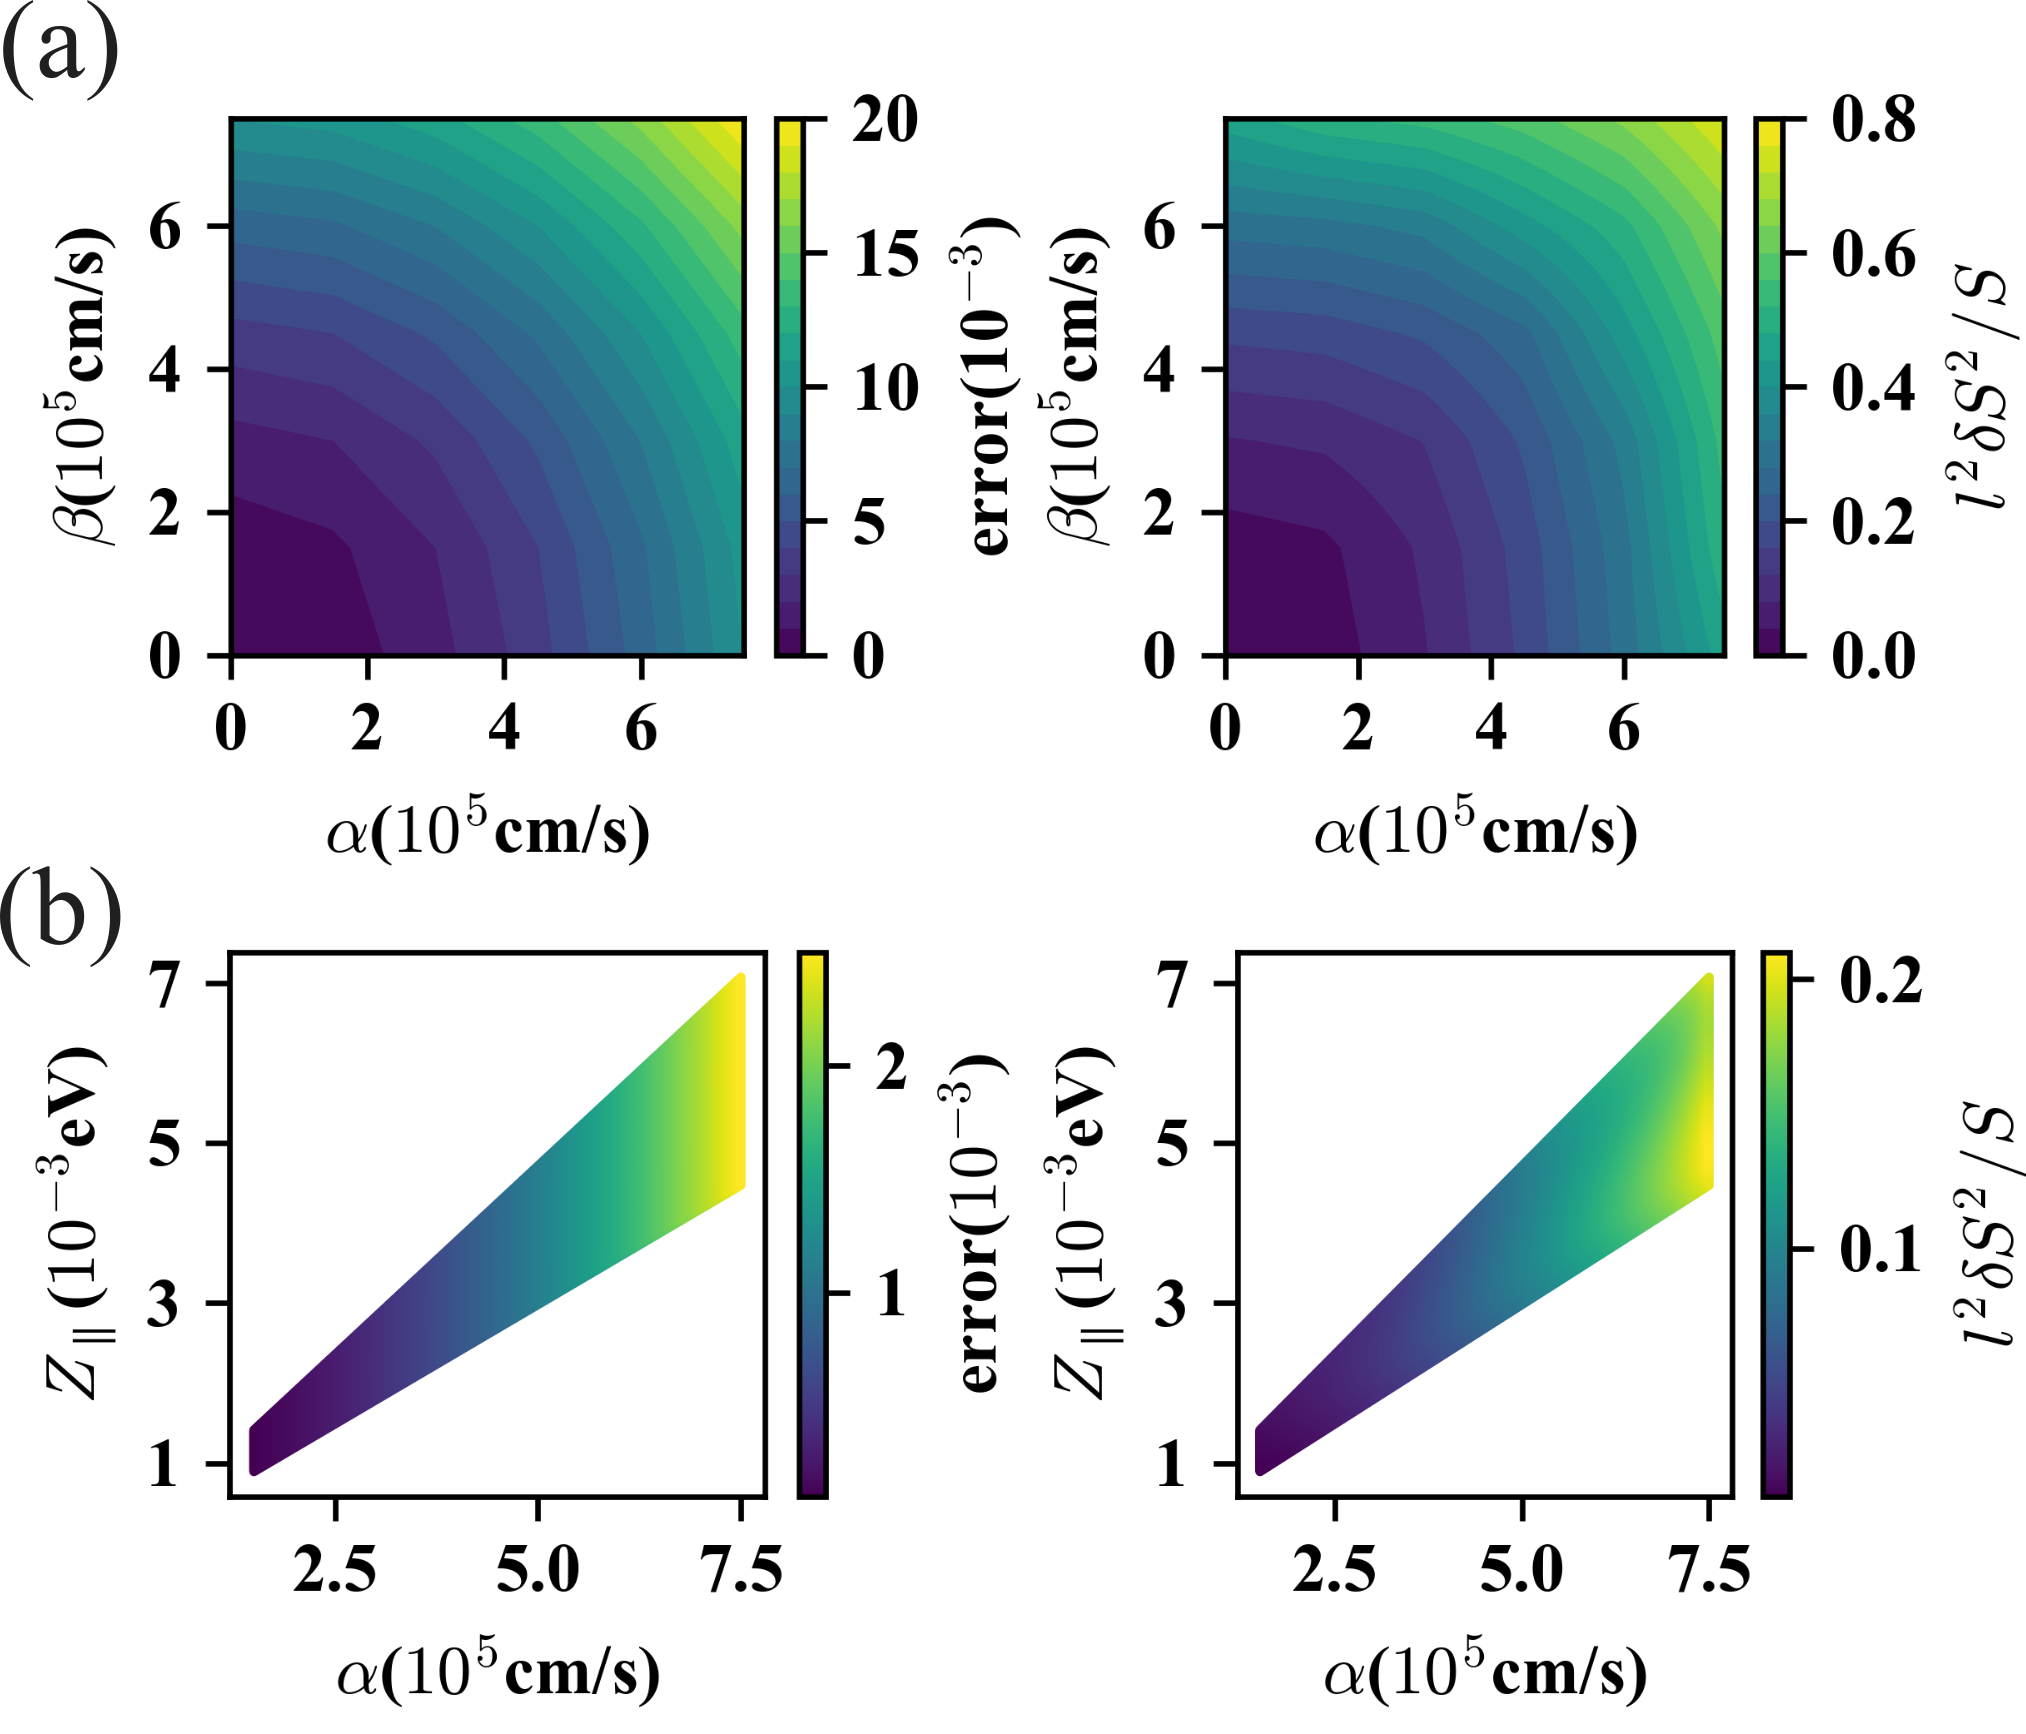
\includegraphics[width=1.0\columnwidth]{error.png}
\caption{{量子化条件和严格对角化的比较。 (a) 对于Rashba-Dresselhaus模型中$(\alpha,\beta)$的各种取值,我们在左边画出了,离$0.4$ eV最近的朗道能级的$\text{error}:=|\epsilon_\text{rule}-\epsilon_\text{exact}|/\var_c$,其中$\epsilon_{\text{exact}}$来自Peierls-Onsager哈密顿量$H_{RD}(\bK)$加上自旋塞曼效应的严格对角化。我们在右边画出了$l^2\delta S^2/S$,可以看出这个量和$\text{error}$有很强的正相关关系。 (b) 对于$H_{RZ}$中的 ($\alpha$, $Z_\parallel$) 的多种取值,我们在左边画出了离$\epsilon_0$【参见\q{whereisdiracpoint}】的朗道能级的误差,对应的$l^2 \delta S^2/S$画在了右边。考虑到数值问题,我们只画出了$0.4{<}\epsilon_0{<}1.0$ eV的部分。(a)的参数: $m=0.076m_0$, $l=200$\AA~以及 $g_{s\perp}=2$; (b)的参数: $m=0.076m_0$, $l=100$\AA~以及 $g_{s\perp}=2$。}\label{fig:error}}
\end{figure}


\section{数值对角化的方法}\label{sec:numerical}

数值对角化依赖于$[K_x,K_y]=il^{-2}$同位置和动量算符的对易关系非常相似。因此,我们可以用产生和湮灭算符来表达$K_x$和$K_y$:
\begin{align}
\begin{split}
K_x=&l^{-1}(a+a^\dagger)/\sqrt{2},\\
K_y=&-il^{-1}(a-a^\dagger)/\sqrt{2}.
\end{split}
\end{align}
在$H_R(\bK)$(加上自旋塞曼项)里用上式的替换
\begin{align}
\begin{split}
H_{R}(\boldsymbol{K})=&\frac{\hbar^2}{ml^2}(a^{\dagger}a+\frac{1}{2})
\\&+\sqrt{2}\hbar\alpha l^{-1}\left(\begin{array}{cc}
0 & -ia^{\dagger}\\
ia & 0
\end{array}\right)
-\frac{g_{s\perp}\hbar^2\sigma^z}{4m_0l^2}.
\end{split}\label{eq:Rashba-ho}
\end{align}
\q{eq:Rashba-ho}有类似于$(c_1|n+1\rangle,c_2|n\rangle)$的解,其中$c_1$和$c_2$是常数,$|n\rangle$是$a^\dagger a$的本征值为$n$的量子态。任意一个哈密顿量$H(\bK)$都可以通过引入$n$的截断来对角化,但是截断需要取得非常大。

\chapter{简并流行的余维数}\label{app:codimension}

\begin{table}
\begin{tabular}{ccccccc}
\hlineB{2}
标识 & $u$ & $s$ & 对称性限制 & $\det{\A}$ & $\breve{g}$ & 余维数 \\
\hline
I-1 & 0 & 0 & $\A=\breve{g}\A\breve{g}^{-1}$ & - & $\breve{g}\propto I$ & 3  \\
&  &  &  & - & $\breve{g} \not\propto I$ & 1  \\
I-2 & 0 & 1 & $\A=\breve{g}\A^*\breve{g}^{-1}$ & 1 & $(\breve{g}K)^2=I$ & 1 \\
&  &  &  & 1 & $(\breve{g}K)^2=-I$ & 3 \\
&  &  &  & -1 & $(\breve{g}K)^2=I$ & $\infty$ \\
&  &  &  & -1 & $(\breve{g}K)^2=-I$ & $\times$ \\
II-1 & 0 & 0 & $\A=\breve{g}(g^{L-1}\circ\bk_0) \A_{1/L}^{L}$ & - & - & 1 \\
II-2 & 1 & 1 & $\A=\breve{g}\A^T\breve{g}^{-1}$ & - & $(\breve{g}K)^2=I$ & 2 \\
& & & & - & $(\breve{g}K)^2\ne I$ & 0 \\
II-3 & 0 & 1 & $\A=\breve{g}(g^{L-1}\circ\bk_0) (K^i\A_{1/L}K^i)^L$ & - & $L=N$ & 1 \\
& & & & 1 & $L\ne N$ & 1 \\
& & & & -1 & $L\ne N$, $(\breve{g}K)^2=I$ & $\infty$ \\
& & & & -1 & $L\ne N$, $(\breve{g}K)^2=-I$ & $\times$ \\
II-4 & 1 & 0 & $\A=\breve{g}\A^\dagger\breve{g}^{-1}$ & 1 &$\breve{g} \propto \sigma_z$& 2\\
& & & & 1 &$\breve{g} \not\propto \sigma_z$ & 0\\
& & & & -1 &$\breve{g} \propto I$ & 2\\
& & & & -1 &$\breve{g} \not\propto I$& 0\\
III-1 & 0 & 0 & $\A_2=\breve{g}\A_1\breve{g}^{-1}$ & - & - & 3 \\
III-2 & 1 & 1 & $\A_2=\breve{g}\A_1^T\breve{g}^{-1}$ & - & - & 3 \\
III-3 & 0 & 1 & $\A_2=\breve{g}\A_1^*\breve{g}^{-1}$ & - & - & 3\\
III-4 & 1 & 0 & $\A_2=\breve{g}\A_1^\dagger\breve{g}^{-1}$ & - & - & 3\\
\hlineB{2}
\end{tabular}
\caption{不同对称性限制下的$\A$的简并流形的余维数。除了II-1和II-3,绝大部分$\A$的对称性约束条件来自于文献\onlinecite{100p}。对于II-1和II-3,我们采用了一个特定的规范。余维数是$\infty$表明$\A$的本征值不可能简并;$\times$表示对于$2\times 2$的$\A$,其对应行标出的$\det\A$和$\breve{g}$不可能同时满足。在倒数第二列,$\breve{g}$要么是对角的,要么是完全非对角的。\label{table:fullcodimension}}
\end{table}

在这个附录里,我们要对$2\times 2$的$\A$【参见\qq{eq:prop}{berryconn}】进行对称性分析,并且推导出其简并的对称性限制的余维数。

对于一个对称操作$g$,其在空间和时间上的变换写为$\br \rightarrow \check{g} \br$和$t\rightarrow (-1)^{s(g)}t$。我们定义$\hat{g}$是对应的算符:$\hat{g} \psi(\br,s)=\sum_{s'}\psi(\check{g}^{-1} \br,s')[D_g]_{s's}$,其中$D_g$是$g$的自旋表示矩阵。缝合矩阵$\breve{g}$的定义是
\e{
   \breve{g}(\bk)_{nm} :\eq \langle u_{n,g\circ\bk}|\hat{g}(\bk)|u_{m,\bk} \rangle K^{s(g)}, \lin
   \hat{g}(\bk):\eq e^{-i\bk\cdot\hat{\br}}\hat{g}e^{i\bk\cdot\hat{\br}}.
}
这里,$n=1,2$, $m=1,2$;$K^1:=K$对应着复共轭,而$K^0$则没有任何操作。在基矢变换下: 
\e{
|u_{n\bk}\rangle \to \sum_{m=1}^2|u_{m\bk}\rangle V_{mn}(\bk),
}
缝合矩阵$\breve{g}$按下式变换
\e{
\breve{g}(\bk) \to V^\dagger(g\circ \bk)\breve{g}(\bk)K^{s(g)}V(\bk)K^{s(g)}.
}
这个变换被称为规范变换。任意的幺正的$\hat{g}$可以通过规范变换对角化,其本征值成为对称性的本征值。我们定义$g$的基数$N$为满足$g^N$为单位元,$2\pi$旋转,晶格平移或者前三者的任意乘积的最小的正整数。

余维数的计算可以通过选择一个方便的规范来简化;当然,余维数是和规范没有关系的。一般而言,我们对$2\times 2$缝合矩阵有如下的规则:
\begin{itemize}
\item 如果$g\circ\bk\ne\bk$, 那么$\breve{g}(\bk)$可以通过规范变换变为单位矩阵。
\item 如果$g\circ\bk=\bk$而且$\hat{g}$是幺正的,那么$\breve{g}(\bk)$可以通过规范变换变为对角阵。
\item 如果$g\circ\bk=\bk$而且$\hat{g}$是反幺正的,那么$\breve{g}(\bk)$可以通过规范变换变为完全非对角阵,完全非对角阵的定义是对角元为零。对于基数为2的$\hat{g}$, $\breve{g}$可以变为$\sigma_x$或者$i\sigma_y$。
\end{itemize}
前两个称述是显然的,而最后一个我们在附录\ref{app:makinggoffdiagonal}中进行了证明。

对称性对$\A$的限制已经在文献\onlinecite{100p}中研究过,我们将结果写在了\tab{table:fullcodimension}中。一般而言,这些限制的推导用到了下面的关系
\e{
&\A[g\circ \bk_f\leftarrow g\circ \bk_i] \nonumber\\
&=e^{i\phi}\breve{g}(\bk_f)K^{s(g)}\A[\bk_f\leftarrow \bk_i]K^{s(g)}\breve{g}^{-1}(\bk_i),\label{eq:propsymm}
}
其中$\A[\bk_f\leftarrow \bk_i]$是从$\bk_i$到$\bk_f$的沿着磁振子轨道的一小段传播子。$e^{i\phi}$是一个由于非点式的操作导致的相位,但是这个相位对整个轨道总是平凡的\cite{100p},因此这里直接略去。

对于十类对称性中的四类III 1-4,对称操作将一个磁振子轨道映射到另外一个磁振子轨道,每个磁振子轨道和自己并没有联系上。因此,余维数仍然是3。对于另外六类,对称性对$\A$有着严格的限制。特别的是,对于I-2, II-3, II-4,$\det(\A)$限制在$\pm 1$\cite{topoferm,100p}。

这六类限制又可以分为两种:(i)将$\A$限制在$\text{SU}(2)$的一个子流形上(I-1, I-2, II-2, II-4);(ii)将$\A$表示为其一部分的乘积【比如\q{eq:sigmazconstraint}】(II-1, II-3)。对前者,我们将$\A$的标准参数化约束到其子流形中,并定义为对称坐标。对于后者,我们采用$\A$的一部分的标准参数化饭干,并定义其为整个$\A$的对称坐标。对于(i),$\A$满足的关系式由$\bk_0$点的缝合矩阵构成,其中$\bk_0$是$\A$的起始点。因此,我们采用
\e{
\A = e^{i\theta}\matrixtwo{\alpha}{\beta}{-\beta^*}{\alpha^*}, |\alpha|^2+|\beta|^2=1.
}
并且研究在加上对称性限制之后还有多少个自由参数。自由参数的数目就是余维数。对于(ii),我们将传播自的第一个小段$\A_{1/L}$参数化
\e{
\A_{1/L} = e^{i\theta}\matrixtwo{\alpha}{\beta}{-\beta^*}{\alpha^*}, |\alpha|^2+|\beta|^2=1.\label{eq:paramA1/N}
}
然后我们计算$\A$并研究要使$\A$正比于单位矩阵,我们需要条件多少个参数。这个参数的数目就是余维数。

\paragraph*{I-1} 根据缝合矩阵的基本性质,我们可以对角化$\breve{g}$得到
\e{
\breve{g} = \matrixtwo{e^{i\phi_1}}{0}{0}{e^{i\phi_2}}.
}
在这个规范里,对称限制是
\e{
\matrixtwo{\alpha}{\beta}{-\beta^*}{\alpha^*}=\matrixtwo{\alpha}{e^{i(\phi_1-\phi_2)}\beta}{-e^{-i(\phi_1-\phi_2)}\beta^*}{\alpha^*}.
}
因此,除非$\breve{g}$正比于单位阵,$\beta=0$,唯一的可变参数是$\alpha$的相位。

\paragraph*{I-2} 通过规范变换,$\breve{g}$可以变成完全非对角的
\e{
\breve{g} = \matrixtwo{0}{1}{\pm 1}{0}.
}
在这个规范内,对称性的限制表达为
\e{
\det({\A})\matrixtwo{\alpha}{\beta}{-\beta^*}{\alpha^*}=\matrixtwo{\alpha}{\mp\beta}{\pm \beta^*}{\alpha^*}.
}
上式直接可以导出\tab{table:fullcodimension}的对应列.

\paragraph*{II-1} 在这一类中(以及II-3),整个的传播子可以用它的$1/L$构造出来,其中$L$是满足$g^L\circ \bk_0=\bk_0$的最小正整数。这里,$\bk_0$是$\A$的起点。在这一类中,$L=N$。$N$重旋转对称性$\mathfrak{c}_{Nz}$就属于这一类。一般而言,通过在$g^n\circ \bk_0$的规范变换,对于$0 \le n < N-1$,$\breve{g}(g^n\circ \bk_0)$可以变成单位阵,而$\A$则成为
\e{
\A=\breve{g}(g^{N-1}\circ\bk_0)\A_{1/N}^N
}
其中
\e{
\breve{g}(g^{N-1}\circ\bk_0)=\prod_{n=0}^{N-1} \breve{g}(g^n\circ\bk_0)
}
是一个由群的乘法表决定的相位因子。比如说如果$g$是$N$重旋转,对于整数(1/2自旋)自旋的系统相位因子就是$+1$($-1$)。根据\q{eq:paramA1/N},我们将$A_{1/N}$对角化 
\e{
A_{1/N} = e^{i\theta}U^{\dagger}\matrixtwo{e^{i\varphi}}{0}{0}{e^{-i\varphi}}U
}
其中$e^{i\varphi}=\text{Re}(\alpha)+i\sqrt{\text{Im}(\alpha)^2+|\beta|^2}$。$A_{1/N}^N \propto I$的充要条件是$\text{Re}(\alpha)=\cos(n\pi/N)$,其中$n$是整数。因此,除了$n=0$和$n=N$需要三个参数之外,其余的$n$都只需要一个参数就可以调到。

在\s{sec:llquasideg}中,我们通过微扰$\mathfrak{c}_\infty$的Rashba模型,或者通过耦合两个原本无关的轨道来构建$\mathfrak{c}_N$的模型。在这两种情况下,如果扰动还没有加上去,$\varphi$是随着$B$单调上升的。因此$\varphi$单调地达到值$n\pi/N$。$e^{i\varphi}$每$N$次取到一次$\pm 1$,因此每$N$个简并中,$N-1$是稳定地,或者说,$N-1$个的余维数是1。

\paragraph*{II-3} 在II-1中,$L=N$。但是,对于II-3,这一点并不一定成立。对于满足$L=N$的对称性,余维数分析和II-1基本相同。而不满足$L\ne N$的对称性只有$T\mathfrak{c}_{6z,n\boldsymbol{c}/6}$ ($n\in\{0,1,2,3,4,5\}$),此时$L=3$而$N=6$。我们此时定义$g=T\mathfrak{c}_{6z,n\boldsymbol{c}/6}$和$h=g^3$。通过规范变换,我们可以使得$\breve{g}(\bk_0)=\breve{g}(g\circ\bk_0)=I$,以及$\breve{h}(\bk_0)=\breve{g}(g^2\circ \bk_0)\equiv\breve{h}$。在这个规范下,$\breve{h}(g\circ\bk_0)=h^*$。因此
\e{
\A=\breve{h}\A_{1/L}\A_{1/L}^*\A_{1/L}
}
而$\A_{1/L}$收到$h$的限制 
\e{
\A_{1/L}=\breve{h}^* \A_{1/L} \breve{h}^{-1}.\label{eq:TC6A1/L}
}
由于$h$的基数是2,$\breve{h}$可以选为$\sigma_x$或$i\sigma_y$。我们立即可以得到$\det \A_{1/L} = \pm 1$。我们首先研究$\breve{h}=\sigma_x$。如果$\det \A_{1/L} = 1$,我们可以按照\q{eq:paramA1/N}参数化$\det \A_{1/L}$,其中$\theta=0$。 根据\q{eq:TC6A1/L},我们得知$\beta=0$,因此 
\e{
\A = \matrixtwo{0}{\alpha^*}{\alpha}{0}
}
并且$\A$本征值的相位被固定为$0$和$\pi$。如果$\det{\A_{1/L}}=-1$,\q{eq:paramA1/N}中$\theta=\pi/2$,我们可以得到
\e{
\A = \matrixtwo{\beta^{*3}}{0}{0}{\beta^3}
}
可见余维数是1。如果$h=i\sigma_y$,根据表格中I-2的第四列,$\det \A_{1/L}=1$。采用\q{eq:paramA1/N}中的参数化($\theta=0$),容易求得余维数是1。

\paragraph*{II-2和II-4} 这两类的计算和I-1和I-2基本相同,在这里略去。

如果我们假设自旋轨道耦合可以连续去除并且不改变简并度,那么I-2, II-3, II-4有$\det(A)=1$。此时表\ref{table:fullcodimension}退化为表\ref{table:codimension-nearlydegen}-\ref{table:codimension-exactlydegen}.

\section{反幺正对称性的$2\times 2$缝合矩阵可以变成完全非对角\label{app:makinggoffdiagonal}}

这里我们推导缝合矩阵规范变换的第三个规则。我们将通过一系列规范变换($\breve{g}\rightarrow \dg{V}\breve{g}V^*$)证明这一点。

\noi{i} 由于反幺正算符的平方是幺正的,因此$\breve{g}\breve{g}^* \rightarrow V^{-1}\breve{g}\breve{g}^*V$可以被对角化。在这个对角化的规范中,很容易看出$\breve{g}$要么是完全非对角的,要么是一个对称的幺正矩阵。如果是前者,证明已经结束,下面我们处理后一种情况。

\noi{ii} 任何对称的幺正矩阵可以用一个实的正交阵来对角化,经过这次变换$\breve{g}$成为对角阵。

\noi{iii} 通过选择合适的对角的$V$,$\breve{g}$可以变为单位矩阵。

\noi{iv} 最后,我们可以用$V=e^{-i(\pi/4)\sigma_x}$得到$\breve{g}=i\sigma_x$,其中$\sigma_x$是一个非对角的泡利矩阵,证明完毕。\\

\end{appendices}

